\documentclass[conference]{IEEEtran}
\usepackage[T1]{fontenc}
\usepackage{amsmath}
\usepackage{graphicx}
\usepackage{booktabs}
\usepackage{tikz}
\usetikzlibrary{arrows.meta,positioning}
\usepackage[hidelinks]{hyperref}
\usepackage{url}
\hypersetup{pdftitle={Pipeline Hazard Detection and Forwarding Unit},pdfauthor={Team Snorlax}}
\begin{document}
\title{Pipeline Hazard Detection and Forwarding Unit}
\author{\IEEEauthorblockN{Ishita Thakur, Aditya Verma, Yug Johri, Anshvardhan, and Swagato Bauri}
\IEEEauthorblockA{Team Snorlax\\Rishihood University, India\\Phase I Project Report --- November 15, 2026}}
\maketitle

\begin{abstract}
Data dependencies can cause a pipelined processor to execute an instruction using an outdated register value. This project develops a modular Verilog hazard-control subsystem for a five-stage educational pipeline. Register comparators detect read-after-write dependencies, a priority forwarding unit selects available EX/MEM or MEM/WB results, and a load-use interlock holds fetch and decode while inserting a bubble into execution. The integration harness supports decoded ADD, SUB, and LW operations and compares forwarding against a functionally correct stall-only baseline. Verification combines 4,194,304 combinational control cases, directed pipeline scenarios, reset and restart testing, and 400 seeded instruction programs. Every valid retirement in the random programs is checked against a sequential reference model. On the ten-instruction directed workload, forwarding reduces execution from 26 to 15 cycles and CPI from 2.600 to 1.500, with one unavoidable load-use stall. A deliberately unprotected mode demonstrates incorrect execution when hazard handling is disabled. Captured waveforms and a reproducible verification target connect the control decisions to observed execution. These results establish simulation-level correctness within the supported instruction subset and memory timing assumptions; they do not claim full ISA compliance or measured FPGA timing.
\end{abstract}
\begin{IEEEkeywords}
pipelining, data hazards, RAW dependencies, operand forwarding, load-use interlock, Verilog, verification
\end{IEEEkeywords}

\section{Introduction}
Pipelining overlaps instruction processing across instruction fetch (IF), register decode (ID), execution (EX), memory access (MEM), and writeback (WB). A consumer can therefore read a register before an older producer reaches WB. For example, ADD r5,r1,r2 followed immediately by SUB r6,r5,r3 must use the newly calculated r5, even though the register file may still contain its old value.

The objective is to preserve sequential execution semantics while avoiding unnecessary stalls. The project implements dependency detection, forwarding selection, operand multiplexing, and controlled bubble insertion as separate modules. A compact five-stage harness makes the behavior observable without the additional complexity of a complete instruction decoder. The design focuses on RAW hazards, ALU dependencies, load-use dependencies, producer priority, and register-zero exclusion.

The prototype is available in a public repository~\cite{repo}. Its contribution is an integrated, reproducible educational implementation with explicit timing assumptions and verification evidence. The forwarding and interlock principles are established techniques; no new processor architecture is claimed.

\section{Literature Review}
\subsection{Forwarding and pipeline timing}
Cornell's CS3410 pipelined Mini-MIPS guidance describes forwarding conditions based on matching producer destinations and consumer sources, write-enable qualification, exclusion of register zero, and producer availability. Its discussion of double hazards prioritizes the more recent EX/MEM producer over MEM/WB~\cite{cornell}. This motivates separate match predicates and explicit priority in the present forwarding unit. A MEM-stage load cannot supply its effective address as the loaded operand.

The CS61C course notes distinguish stalling from bypassing and explain the timing of MEM-to-EX and WB-to-EX paths. They also discuss same-cycle register-file write/read behavior and why a load immediately followed by a consumer can still require a bubble~\cite{berkeley}. Our integration states this timing contract directly: WB-to-ID bypass is explicit, and memory data becomes usable by the following consumer through MEM/WB after one stall.

\subsection{Systematic dependency coverage}
Mahran presents a method for enumerating dependency cases using instruction operand information and the stages at which data is read or produced~\cite{mahran}. This supports treating source-use flags and result availability as part of hazard detection, rather than comparing every instruction field indiscriminately. In this prototype, LW uses rs1 as its base but does not use rs2. The verification plan therefore includes both true dependencies and aliases in unused fields.

The RISC-V RV32I specification defines 32 integer registers and a hardwired-zero x0~\cite{riscv}. The prototype uses corresponding 5-bit register identifiers and zero-register behavior as a convenient teaching convention. Its decoded operations, word-indexed memory, and simplified immediates are not a claim of RV32I compatibility. Icarus Verilog documentation distinguishes simulation and synthesis and describes the compiler/runtime workflow~\cite{icarus}; this project reports simulation evidence rather than technology-specific implementation results.

\section{Proposed Solution}
\subsection{Pipeline and module organization}
Fig.~\ref{fig:architecture} shows the integration. Each pipeline stage carries a valid bit so an inserted bubble cannot write a register or retire. The standalone control modules are combinational Verilog. The harness supplies decoded instruction arrays and simulation memory.

\begin{figure}[t]
\centering
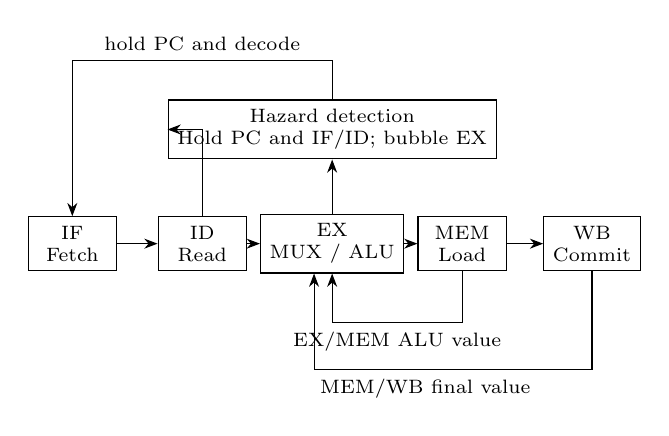
\begin{tikzpicture}[x=1cm,y=1cm,>=Stealth,font=\scriptsize,
 stage/.style={draw,minimum width=1.12cm,minimum height=.65cm,align=center}]
\node[stage] (if) at (0,0) {IF\\Fetch};
\node[stage] (id) at (1.65,0) {ID\\Read};
\node[stage] (ex) at (3.3,0) {EX\\MUX / ALU};
\node[stage] (mem) at (4.95,0) {MEM\\Load};
\node[stage] (wb) at (6.6,0) {WB\\Commit};
\draw[->] (if)--(id);\draw[->] (id)--(ex);\draw[->] (ex)--(mem);\draw[->] (mem)--(wb);
\draw[->] (mem.south)--++(0,-.65)-|node[pos=.25,below]{EX/MEM ALU value}(ex.south);
\draw[->] (wb.south)--++(0,-1.25)-|node[pos=.3,below]{MEM/WB final value}([xshift=-.23cm]ex.south);
\node[draw,align=center,minimum width=2.9cm] (h) at (3.3,1.45) {Hazard detection\\Hold PC and IF/ID; bubble EX};
\draw[->] (id.north)|-(h.west);\draw[->] (ex.north)--(h.south);
\draw[->] (h.north)--++(0,.5)-|node[pos=.25,above]{hold PC and decode}(if.north);
\end{tikzpicture}
\caption{Five-stage integration and two operand-forwarding paths. The hazard unit observes register metadata, controls fetch/decode holds, and invalidates the next EX slot. WB-to-ID bypass is also implemented.}
\label{fig:architecture}
\end{figure}

\texttt{register\_match.v} compares a used source against a nonzero destination with an asserted write enable. \texttt{forwarding\_unit.v} selects a producer independently for each ALU operand. \texttt{forward\_mux.v} routes the captured ID/EX value, final WB value, or MEM ALU value. \texttt{hazard\_detection.v} detects the load-use interlock or the broader stall-only dependencies. \texttt{stall\_control.v} generates PC write, IF/ID write, and ID/EX flush signals. \texttt{pipeline\_demo.v} integrates these blocks.

The 32-bit register fixture initializes rN to N, with r0 fixed at zero. ADD and SUB use two sources; LW calculates base plus an immediate and reads one of 256 data words using the low eight address bits. The testbench initializes memory. Reset is synchronous and active high. Stores, branches, binary instruction decoding, caches, and variable-latency memory are outside the supported scope.

\subsection{Dependency predicates and priority}
For a source $s$ and producer $p$, the dependency predicate is
\begin{equation}
D(s,p)=U_s\land W_p\land(rd_p\ne0)\land(rs_s=rd_p),
\end{equation}
where $U_s$ indicates that the source is actually consumed and $W_p$ includes the producer's valid/write qualification. A valid MEM match selects EX/MEM first if it is not a load. Otherwise, a valid WB match can select the final MEM/WB value. Table~\ref{tab:select} defines the mux encoding.

\begin{table}[t]
\caption{Forwarding Mux Encoding}
\label{tab:select}\centering
\begin{tabular}{cl}
\toprule Selector & Operand source\\\midrule
00 & Captured ID/EX register value\\
01 & MEM/WB final writeback value\\
10 & EX/MEM ALU result\\
11 & Reserved; falls back to captured value\\\bottomrule
\end{tabular}
\end{table}

A newer MEM load masks an older WB match to the same destination. Forwarding that older value would violate program order. The pipeline interlock prevents the dependent instruction from entering EX until the load's final data is available; the mux does not forward a memory address as loaded data.

\subsection{Load-use stall and bubble insertion}
Let $L_{EX}$ denote a valid EX load, and $D_1,D_2$ the ID source matches against its destination. In forwarding mode,
\begin{equation}
S=L_{EX}\land(D_1\lor D_2).
\end{equation}
The source-use mask disables $D_2$ for LW. The control outputs are
\begin{equation}
\begin{aligned}
PCWrite &= IFIDWrite = \neg S,\\
IDEXFlush &= S.
\end{aligned}
\end{equation}
When $S=1$, PC and IF/ID hold, the next ID/EX slot becomes invalid, and older stages advance. After one bubble, the dependent consumer reaches EX when the loaded value is in MEM/WB. Explicit WB-to-ID bypass defines same-cycle register write/read semantics.

Three harness modes separate correctness and performance: MODE=0 uses stall-only RAW interlocks for EX and MEM dependencies; MODE=1 uses forwarding plus load-use stalls; MODE=2 deliberately disables both. Only the first two modes are intended to execute dependent programs correctly. Invalid slots clear result/load metadata and do not trigger data-memory reads.

\section{Verification Methodology}
The complete local audit runs with \texttt{make verify} using Icarus Verilog 13.0, its \texttt{vvp} runtime, Make, and Python 3. No external Python package is needed for RTL verification. The report build is independent of simulation.

The combinational sweep checks every source/MEM/WB register triple for each operand, all 64 combinations of source-use, write, load, and hazard-mode controls, and two source-pair patterns: complementary IDs and equal IDs. This gives $32^3\times64\times2=4{,}194{,}304$ tested combinations. The mux's reserved selector is checked separately. This is broad input coverage of the specified blocks, not an enumeration of every possible processor state.

Directed integration compares all 32 architectural registers with a sequential model. Nine additional scenarios cover independent instructions, unused LW rs2 fields, load-to-r0, a load consumed as operand B, a load used as another load's base, simultaneous WB/MEM forwarding to different operands, repeated load destinations, and a newer load replacing an older ALU producer. A clock-edge assertion checks fetch/decode hold and EX bubble insertion. A reset test interrupts an active load-use dependency, clears state, and checks a clean restart.

Four deterministic seeds generate 400 programs of 64 instructions each, with dependency-biased ADD, SUB, and LW streams. Each of the 25,600 instructions is executed in both protected modes, giving 51,200 checked retirements. The scoreboard compares every retirement destination and value with an independent sequential model, then checks all final registers. Timeouts, cycle accounting, retirement counts, and stable completion counters are also checked. Case-inequality assertions reject unknown values rather than allowing them to escape timing checks.

\section{Results and Discussion}
\subsection{Directed workload and CPI}
Both protected modes retire the same ten instructions and match the sequential reference. Table~\ref{tab:cpi} gives captured simulation results. Four pipeline fill/drain cycles are included, so $C=N+4+S$ and $CPI=C/N$ for this fixed-latency harness.

\begin{table}[t]
\caption{Ten-Instruction Directed Benchmark}
\label{tab:cpi}\centering
\begin{tabular}{lrrr}
\toprule Mode & Cycles & Stalls & CPI\\\midrule
Forwarding and interlock & 15 & 1 & 1.500\\
Stall-only interlocks & 26 & 12 & 2.600\\\bottomrule
\end{tabular}
\end{table}

The cycle reduction is $(26-15)/26=42.3\%$, and the cycle-based speedup is $26/15=1.73\times$. These numbers apply to this dependency-heavy workload at an assumed equal clock period. No synthesis measurement establishes an equal maximum frequency, area overhead, power reduction, or speedup on general applications.

A separate four-instruction comparison demonstrates why correctness must precede CPI interpretation. ADD r5,r1,r2 followed by SUB r6,r5,r3 produces r6=0 with protected modes. The unprotected mode uses stale r5=5 and produces r6=2. Forwarding completes in eight cycles, stall-only in ten, and the incorrect unprotected execution in eight. Thus a low cycle count alone does not establish a useful optimization.

\subsection{Waveforms and regression evidence}
The VCD audit checks five events in the captured directed waveform: EX/MEM forwarding to operand A at 50 ns; MEM/WB forwarding to operand B at 60 ns; newest-producer selection on both operands at 90 ns; load-use detection at 100 ns; and loaded-data forwarding at 120 ns. At 110 ns, EX is invalid and PC remains held at 8. Table~\ref{tab:wave} isolates that stall sequence. Times are stable testbench samples, not physical propagation-delay measurements.

\begin{table}[t]
\caption{Captured Load-Use Sequence}
\label{tab:wave}\centering
\begin{tabular}{rrrrl}
\toprule Time (ns) & PC & EX valid & Stall & Observation\\\midrule
100 & 8 & 1 & 1 & Load in EX\\
110 & 8 & 0 & 0 & Bubble; PC held\\
120 & 9 & 1 & 0 & WB operand A = 103\\\bottomrule
\end{tabular}
\end{table}

All four random seeds pass. Aggregated over 100 programs per seed, forwarding cycles are 7,706, 7,677, 7,706, and 7,711; stall-only cycles are 12,258, 12,371, 12,299, and 12,303, respectively. These totals include fill/drain overhead for every program. The seeds are 1511506142, 1, 42, and 20261114. Raw logs, CSV measurements, and VCD files accompany the implementation~\cite{repo}.

\section{Individual Contributions}
The team allocates responsibility across the following workstreams. This division identifies the parts each member owns and should be prepared to explain; individual GitHub evidence is maintained separately from role allocation.

\textbf{Ishita Thakur:} Five-stage pipeline integration, valid-bit flow, stage interfaces, and coordination of the integrated prototype.

\textbf{Aditya Verma:} Register-ID comparison, forwarding operand multiplexers, and forwarding-selection interfaces.

\textbf{Yug Johri:} Core hazard-control logic, load-use detection, PC and IF/ID holds, EX bubble insertion, and explanation of the stall sequence.

\textbf{Anshvardhan:} Directed and randomized verification, retirement scoreboards, reset testing, and review of waveform assertions.

\textbf{Swagato Bauri:} Result tabulation, CPI analysis, literature references, and report organization.

Each member is responsible for explaining the relevant RTL, tests, and design decisions during evaluation. Workstream allocation and independently attributable repository changes are separate forms of evidence; both should reflect the team's actual work.

\section{Conclusion and Next Steps}
The prototype implements the requested hazard-detection and forwarding functions within a stated five-stage timing model. Protected execution agrees with the reference model across the directed, edge, reset, and seeded regression suites. Forwarding removes avoidable ALU dependency stalls while retaining the required load-use bubble. The submitted artefacts provide a reproducible connection between RTL conditions, waveform events, and CPI results.

Phase II can extend the harness with stores, branch control, a binary decoder, variable-latency memory, formal properties, and synthesis-based timing/area measurements. The present evidence supports simulation correctness for ADD, SUB, and LW under fixed memory latency; a full processor or hardware implementation would require additional verification.

\begin{thebibliography}{00}
\bibitem{repo} Team Snorlax, ``Pipeline Hazard Detection and Forwarding Unit,'' source repository and simulation evidence, Nov. 2026. [Online]. Available: \url{https://github.com/Mystic-commits/pipeline-hazard-unit}. Accessed: Nov. 15, 2026.
\bibitem{cornell} Cornell University, ``Project 3: Pipelined Mini-MIPS,'' CS3410, Fall 2016. [Online]. Available: \url{https://www.cs.cornell.edu/courses/cs3410/2016fa/projects/p3/}. Accessed: Nov. 15, 2026.
\bibitem{berkeley} CS 61C Course Staff, ``Data Hazards,'' CS 61C Course Notes. [Online]. Available: \url{https://notes.cs61c.org/content/pipeline-hazards/data-hazards/}. Accessed: Nov. 15, 2026.
\bibitem{mahran} A. M. Mahran, ``A handy systematic method for data hazards detection in an instruction set of a pipelined microprocessor,'' arXiv:1203.0787, Mar. 2012, doi: 10.48550/arXiv.1203.0787.
\bibitem{riscv} RISC-V International, ``RV32I Base Integer Instruction Set, Version 2.1,'' \emph{The RISC-V Instruction Set Manual}, vol. I, 2024. [Online]. Available: \url{https://docs.riscv.org/reference/isa/v20240411/unpriv/rv32.html}. Accessed: Nov. 15, 2026.
\bibitem{icarus} Icarus Verilog Contributors, ``Simulation Using Icarus Verilog,'' Icarus Verilog documentation. [Online]. Available: \url{https://steveicarus.github.io/iverilog/usage/simulation.html}. Accessed: Nov. 15, 2026.
\end{thebibliography}
\end{document}
